\documentclass{report}
\usepackage[T1]{fontenc}
\usepackage{graphicx}

\title{Aktien-Ticker}
\author{Pius Rauch}

\begin{document}
\maketitle

\chapter{Einführung}

\section{Teamaufgabe 1}

Unser Projekt „Aktien-Ticker“ zeigt Aktienkurse in Echtzeit und nutzt KI für Prognosen.  
Das Backend wird mit Java entwickelt, das Frontend mit HTML, CSS und JavaScript.  
Ein Video-Slider zeigt Kursbewegungen, und eine App bietet QR-Code-gestützte Funktionen.  
Die OpenAI-API analysiert historische Daten zur Vorhersage von Trends.  
Das Team: Paul Summerauer (Backend/Projektleiter), Pius Rauch (Frontend), Fabian Holzknecht (Design/Backend).  

\section{Teamaufgabe 2}

Die Entwicklung beginnt mit der Planung der Geschäftslogik.  
Danach folgen API-Integration, Frontend- und Backend-Entwicklung.  
Ein Schulserver wird genutzt, um Daten und Medien bereitzustellen.  
Regelmäßige Tests und Nutzerfeedback verbessern die Anwendung.  
Das Projekt endet mit der Präsentation und Dokumentation im Juni 2025.  

\section{Teamaufgabe 3}

Der Fokus liegt auf der Optimierung und finalen Umsetzung.  
Fehlende Features werden ergänzt, Performance verbessert und das Design finalisiert.  
Tests mit Nutzern stellen sicher, dass alle Funktionen stabil laufen.  
Das Projekt wird dokumentiert und für die Präsentation vorbereitet.  

PSP
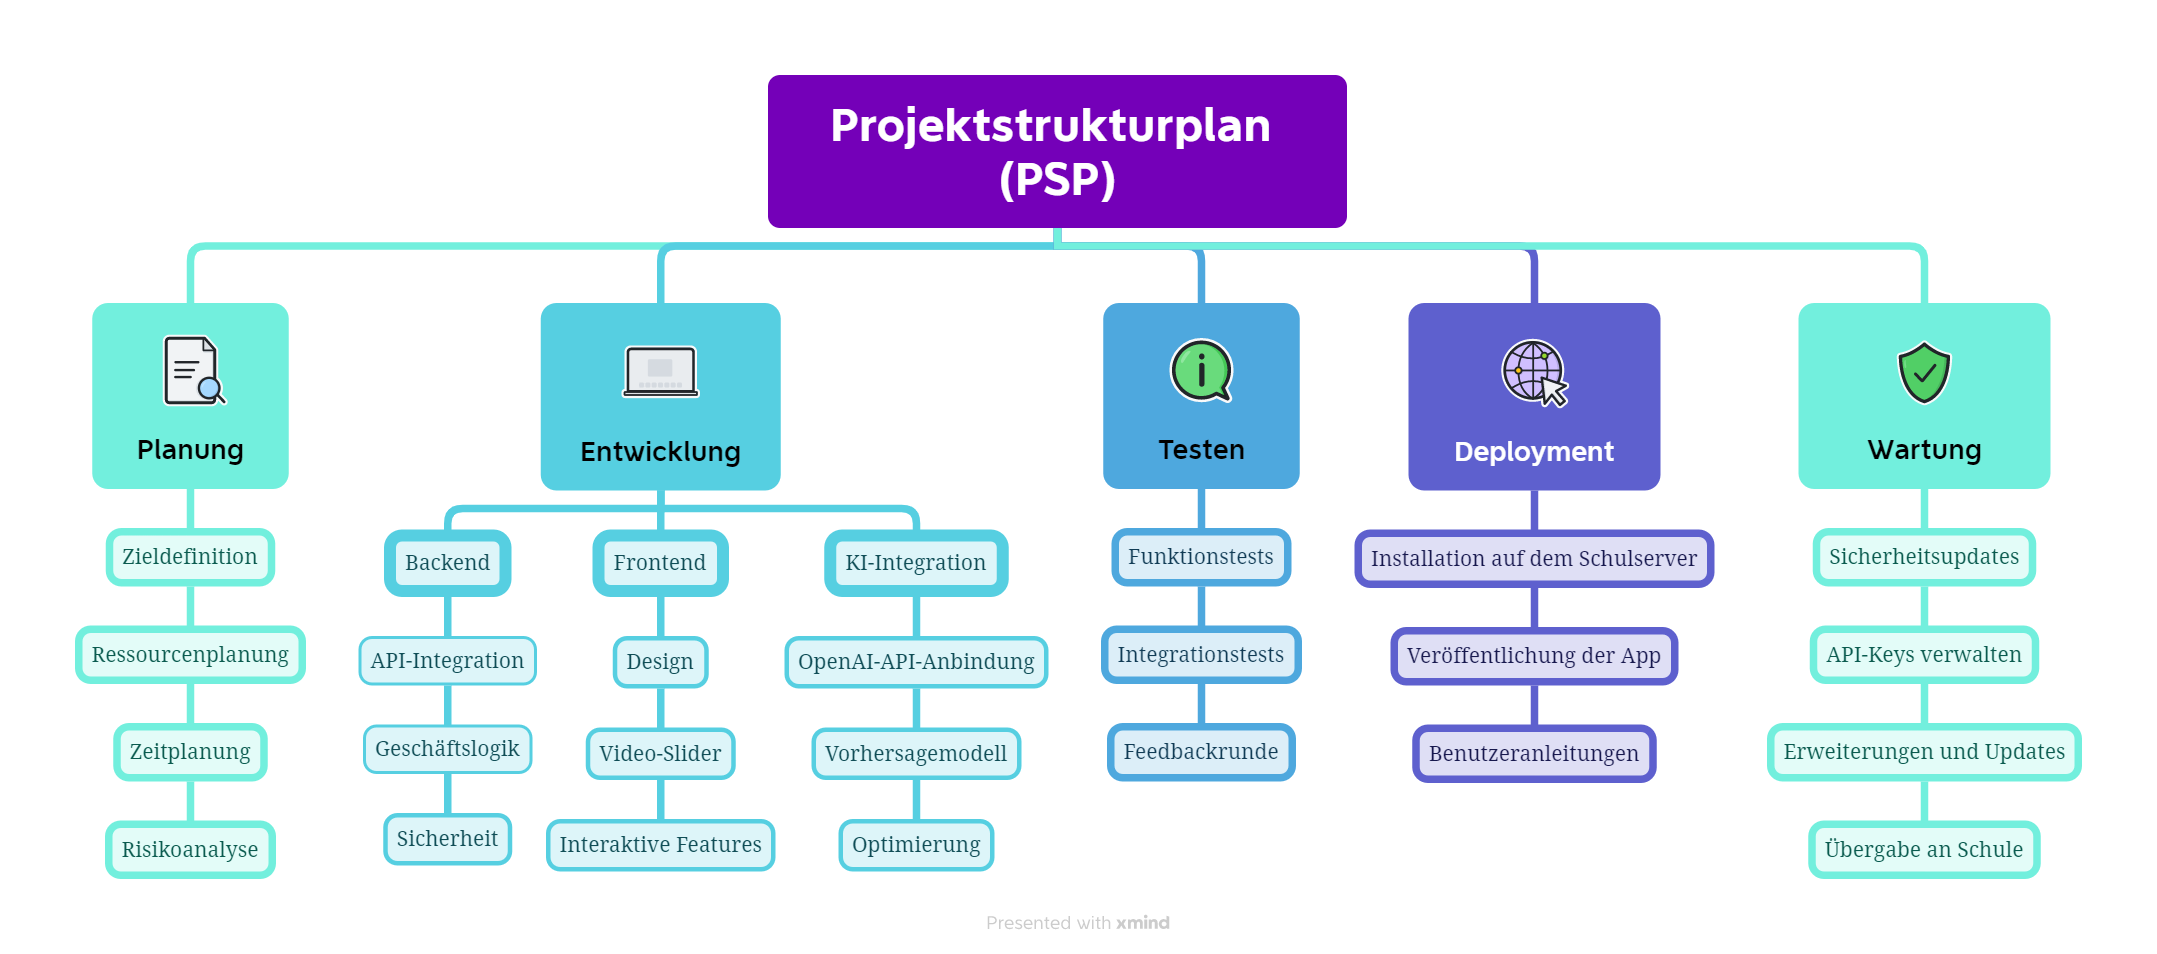
\includegraphics[width=0.75\textwidth]{Projektstrukturplan.png}
In Abb. \ref{fig:PSP} ist der Projektstrukturplan zu sehen
Risikomatrix
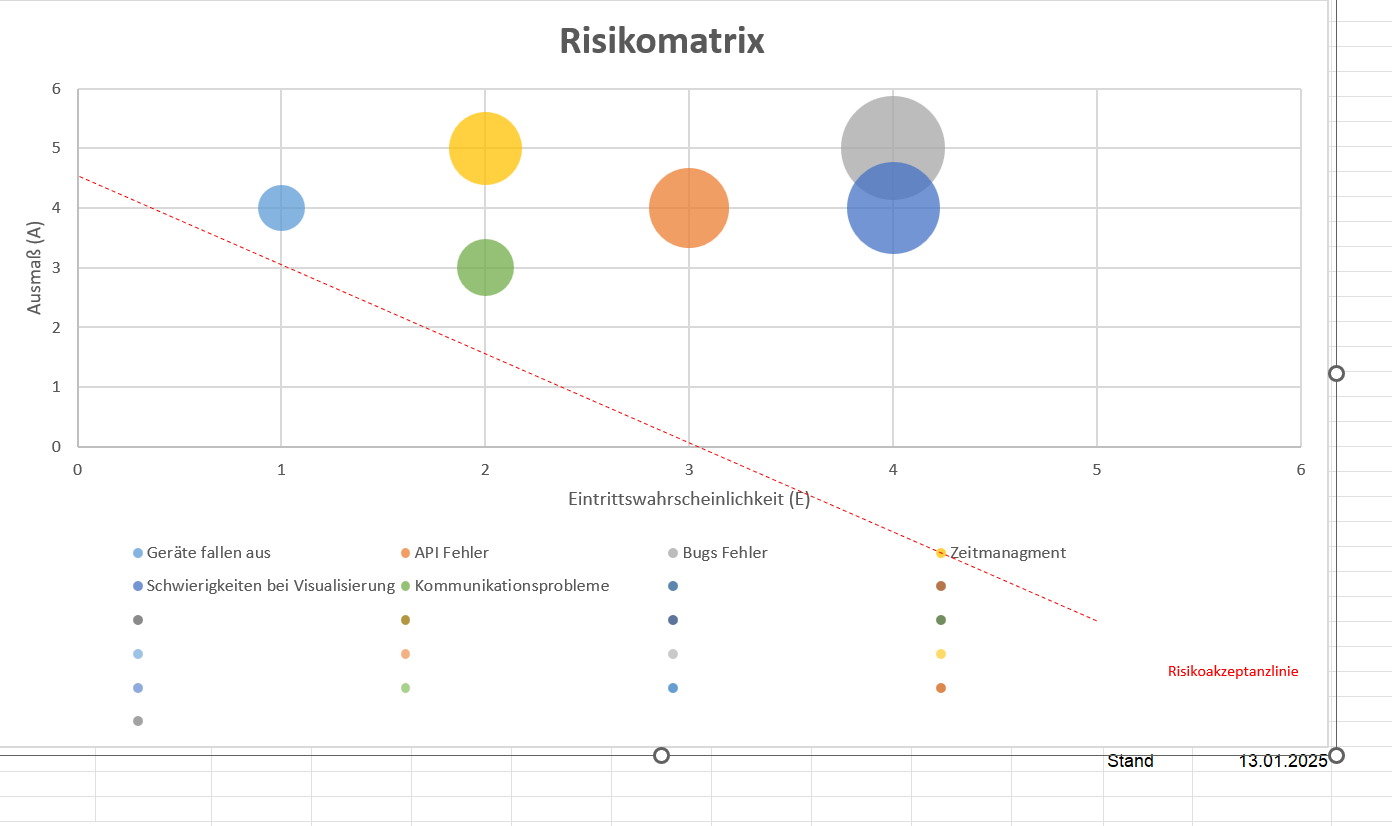
\includegraphics[width=0.75\textwidth]{Risikomatrix.png}
Abb. \ref{fig:Risikomatrix} ist die Risikomatrix abgebildet.
\section{Teamaufgabe 4}

Die letzten Neuerungen umfassen die vollständige Umsetzung des Frontends mit HTML und CSS.  
Der Video-Slider wurde integriert, der alle 15 Sekunden zwischen den Kursdaten wechselt.  
Die API-Integration zur Anzeige von Echtzeit-Aktienkursen wurde abgeschlossen.  
Die OpenAI-API zur Vorhersage von Kursbewegungen wurde eingebunden, und die ersten Analysen laufen.  
QR-Codes für die Mobile-App und Benachrichtigungsfunktionen wurden vorbereitet.  
In den nächsten Schritten werden Frontend und Backend zusammengeführt, und die Anwendung wird umfassend getestet.
\end{document}

